% Laporan: Friendly numbers
\documentclass[12pt,a4paper]{article}
\usepackage[utf8]{inputenc}
\usepackage[T1]{fontenc}
\usepackage[indonesian]{babel}
\usepackage{geometry}
\usepackage{hyperref}
\usepackage{amsmath,amssymb}
\usepackage{listings}
\usepackage{xcolor}
\usepackage{graphicx}
\usepackage{algorithm}
\usepackage{algorithmic}
\usepackage[ruled,vlined,linesnumbered]{algorithm2e}
\geometry{margin=1in}

% --- Definisi warna untuk syntax highlighting ---
\definecolor{codebg}{rgb}{0.97,0.97,0.97}
\definecolor{keyword}{RGB}{0,0,180}
\definecolor{comment}{RGB}{0,128,0}
\definecolor{string}{RGB}{163,21,21}
\definecolor{number}{RGB}{128,0,128}
\definecolor{identifier}{RGB}{0,0,0}

% --- Bahasa dan format untuk C++ ---
\lstdefinelanguage{C++}{
  morekeywords={
    alignas,alignof,and,and_eq,asm,auto,bitand,bitor,bool,break,case,catch,char,
    char8_t,char16_t,char32_t,class,compl,const,const_cast,continue,decltype,default,delete,do,double,
    dynamic_cast,else,enum,explicit,export,extern,false,float,for,friend,goto,if,inline,int,long,
    mutable,namespace,new,noexcept,not,not_eq,nullptr,operator,or,or_eq,private,protected,public,
    register,reinterpret_cast,return,short,signed,sizeof,static,static_assert,static_cast,struct,switch,
    template,this,thread_local,throw,true,try,typedef,typeid,typename,union,unsigned,using,virtual,void,
    volatile,wchar_t,while,xor,xor_eq,pair,printf,scanf,EOF
  },
  sensitive=true,
  morecomment=[l]{//},
  morecomment=[s]{/*}{*/},
  morestring=[b]",
  morestring=[b]',
  alsoletter={_},
}

% --- Gaya umum untuk listing ---
\lstset{
  language=C++,
  backgroundcolor=\color{codebg},
  basicstyle=\ttfamily\small,
  keywordstyle=\color{keyword}\bfseries,
  commentstyle=\color{comment}\itshape,
  stringstyle=\color{string},
  numberstyle=\tiny\color{number},
  identifierstyle=\color{identifier},
  numbers=left,
  stepnumber=1,
  numbersep=8pt,
  tabsize=2,
  showspaces=false,
  showstringspaces=false,
  frame=single,
  breaklines=true,
  captionpos=b
}

\title{Laporan Penyelesaian Soal ``Friendly Numbers''}
\author{Gilbran Mahdavikia Raja \\ 5025241134}

\begin{document}
\maketitle

\begin{abstract}
Laporan ini menjelaskan penyelesaian masalah \emph{Friendly numbers} (sering juga disebut \emph{amicable pairs}) yang meminta kita menemukan semua pasangan bilangan berbeda \(a, b\) dalam interval \([M, N]\) sehingga jumlah pembagi \(a\) (selain \(a\) sendiri) sama dengan \(b\) dan sebaliknya. Dokumentasi memuat deskripsi masalah, strategi solusi yang digunakan (menggunakan daftar pasangan prekomputasi), analisis kompleksitas, kode penyelesaian C++, serta penjelasan pengujian dan kesimpulan.
\end{abstract}

\section{Pemahaman Masalah}
Dua bilangan natural berbeda disebut \emph{friendly} (amicable) jika:
\[
\sigma(a) - a = b \quad\text{dan}\quad \sigma(b) - b = a,
\]
dengan \(\sigma(x)\) adalah jumlah semua pembagi positif \(x\). Kita diminta mencetak semua pasangan \((a, b)\) dengan \(M \le a < b \le N\). Jika tidak ada pasangan dalam interval, keluarkan ``Absent''.

\noindent
\textbf{Batasan:}
\begin{itemize}
  \item \(1 \le M \le N \le 1{,}000{,}000\)
  \item Batas waktu eksekusi: 1 detik
  \item Batas memori: 64 MB
\end{itemize}

\section{Contoh Input / Output}
\textbf{Contoh}
\begin{verbatim}
Input:
200 300

Output:
220 284
\end{verbatim}

\section{Pendekatan Solusi}
Untuk rentang atas \(N \le 10^6\), telah diketahui daftar pasangan bilangan \emph{amicable} dari hasil penelitian matematis. Pendekatan yang digunakan adalah memanfaatkan daftar pasangan tersebut dalam bentuk array prekomputasi, lalu mencetak semua pasangan yang keduanya berada di interval \([M, N]\).

\subsection{Keuntungan}
\begin{itemize}
  \item Eksekusi sangat cepat karena hanya memeriksa sejumlah pasangan tetap (konstanta).
  \item Menghemat waktu dan memori.
\end{itemize}

\subsection{Kekurangan}
\begin{itemize}
  \item Ketergantungan pada kelengkapan daftar prekomputasi.
  \item Tidak bersifat generik jika batas \(N\) diperluas.
\end{itemize}

\subsection{Alternatif Pendekatan}
Jika tidak ingin menggunakan data prekomputasi, kita bisa menghitung fungsi \(\sigma(x)-x\) (sum of proper divisors) untuk semua \(x\) hingga \(N\) dengan metode seperti \textit{sieve}:
\begin{enumerate}
  \item Inisialisasi array \(s[i] = 1\) untuk semua \(i > 1\).
  \item Untuk setiap \(d\) dari 2 hingga \(N/2\), tambahkan \(d\) ke semua kelipatan \(k = 2d, 3d, \ldots\).
  \item Setelah semua nilai \(s[i]\) dihitung, cek semua \(a\): bila \(b = s[a]\) dan \(s[b] = a\), maka pasangan \((a, b)\) adalah amicable.
\end{enumerate}
Kompleksitasnya sekitar \(O(N \log N)\), masih dapat diterima untuk \(N = 10^6\).

\section{Analisis Kompleksitas}
\textbf{Pendekatan prekomputasi:}
\begin{itemize}
  \item Waktu: \(O(K)\), di mana \(K\) jumlah pasangan dalam daftar (konstanta \(\approx 40\)).
  \item Memori: \(O(K)\), sangat kecil.
\end{itemize}

\textbf{Pendekatan sieve:}
\begin{itemize}
  \item Waktu: \(O(N \log N)\).
  \item Memori: \(O(N)\) untuk array jumlah pembagi.
\end{itemize}

\section{Algoritma}

\begin{algorithm}[H]
\caption{Menemukan Pasangan Friendly Numbers dalam Interval [M, N]}
\SetAlgoLined
\KwIn{Bilangan bulat $M$ dan $N$ ($1 \le M \le N \le 10^6$)}
\KwOut{Semua pasangan $(a,b)$ yang bersahabat dalam interval tersebut atau \texttt{Absent}}
\BlankLine
\textbf{Langkah 1:} Inisialisasi array \texttt{arr} berisi pasangan bilangan amicable yang sudah diketahui.

\textbf{Langkah 2:} Baca nilai $M$ dan $N$ dari input.

\textbf{Langkah 3:} \ForEach{pasangan $(x, y)$ dalam \texttt{arr}}{
  \If{$M \le x \le N$ dan $M \le y \le N$}{
    Cetak $x$, $y$
    
    \texttt{found} $\leftarrow$ true
  }
}
\textbf{Langkah 4:} \If{\texttt{found} = false}{
  Cetak \texttt{Absent}
}
\end{algorithm}

\section{Kode Penyelesaian}
Berikut kode C++ solusi dengan daftar pasangan prekomputasi:
\begin{lstlisting}
#include <iostream>
using namespace std;

pair<int, int> arr[] = {
    {220, 284}, {1184, 1210}, {2620, 2924},
    {5020, 5564}, {6232, 6368}, {10744, 10856},
    {12285, 14595}, {17296, 18416}, {63020, 76084}, 
    {66928, 66992}, {67095, 71145}, {69615, 87633},
    {79750, 88730}, {100485, 124155}, {122265, 139815}, 
    {122368, 123152}, {141664, 153176}, {142310, 168730},
    {171856, 176336}, {176272, 180848}, {185368, 203432}, 
    {196724, 202444}, {280540, 365084}, {308620, 389924}, 
    {319550, 430402}, {356408, 399592}, {437456, 455344}, 
    {469028, 486178}, {503056, 514736}, {522405, 525915}, 
    {600392, 669688}, {609928, 686072}, {624184, 691256}, 
    {635624, 712216}, {643336, 652664}, {667964, 783556}, 
    {726104, 796696}, {802725, 863835}, {879712, 901424}, 
    {898216, 980984}
  };

int main() {
  int m, n;
  while (scanf("%d %d", &m, &n) != EOF) {
    bool found = false;
    for (int i = 0; i < 40; i++) {
      if (m <= arr[i].first && arr[i].first <= n &&
          m <= arr[i].second && arr[i].second <= n) {
        printf("%d %d\n", arr[i].first, arr[i].second);
        found = true;
      }
    }
    if (!found) printf("Absent");
  }
  return 0;
}
\end{lstlisting}

\section{Penjelasan Kode}
\begin{itemize}
  \item Array \texttt{arr[]} menyimpan pasangan-pasangan amicable yang sudah diketahui.
  \item Program membaca dua bilangan \(m, n\) (bisa beberapa test case sampai EOF).
  \item Setiap pasangan dicek apakah keduanya berada dalam interval \([m,n]\).
  \item Bila tidak ditemukan pasangan, program mencetak \texttt{Absent}.
\end{itemize}

\section{Contoh Eksekusi}
\begin{verbatim}
Input:
200 300

Output:
220 284
\end{verbatim}
Pasangan 220 dan 284 memenuhi definisi:
\[
\sigma(220)-220 = 284,\quad \sigma(284)-284 = 220
\]

\section{Kasus Tepi dan Penanganan}
\begin{itemize}
  \item Jika \(M=N\) atau interval sangat kecil, hasil kemungkinan \texttt{Absent}.
  \item Bila interval di luar jangkauan tabel, hasil bisa kosong.
  \item Program menangani banyak input berurutan hingga EOF.
\end{itemize}

\section{Kesimpulan}
Pendekatan prekomputasi terbukti efisien, sederhana, dan sesuai batas waktu 1 detik.  
Untuk jangkauan lebih luas, bisa digunakan metode sieve untuk menghitung jumlah pembagi secara dinamis.

\section{Bukti Submission}
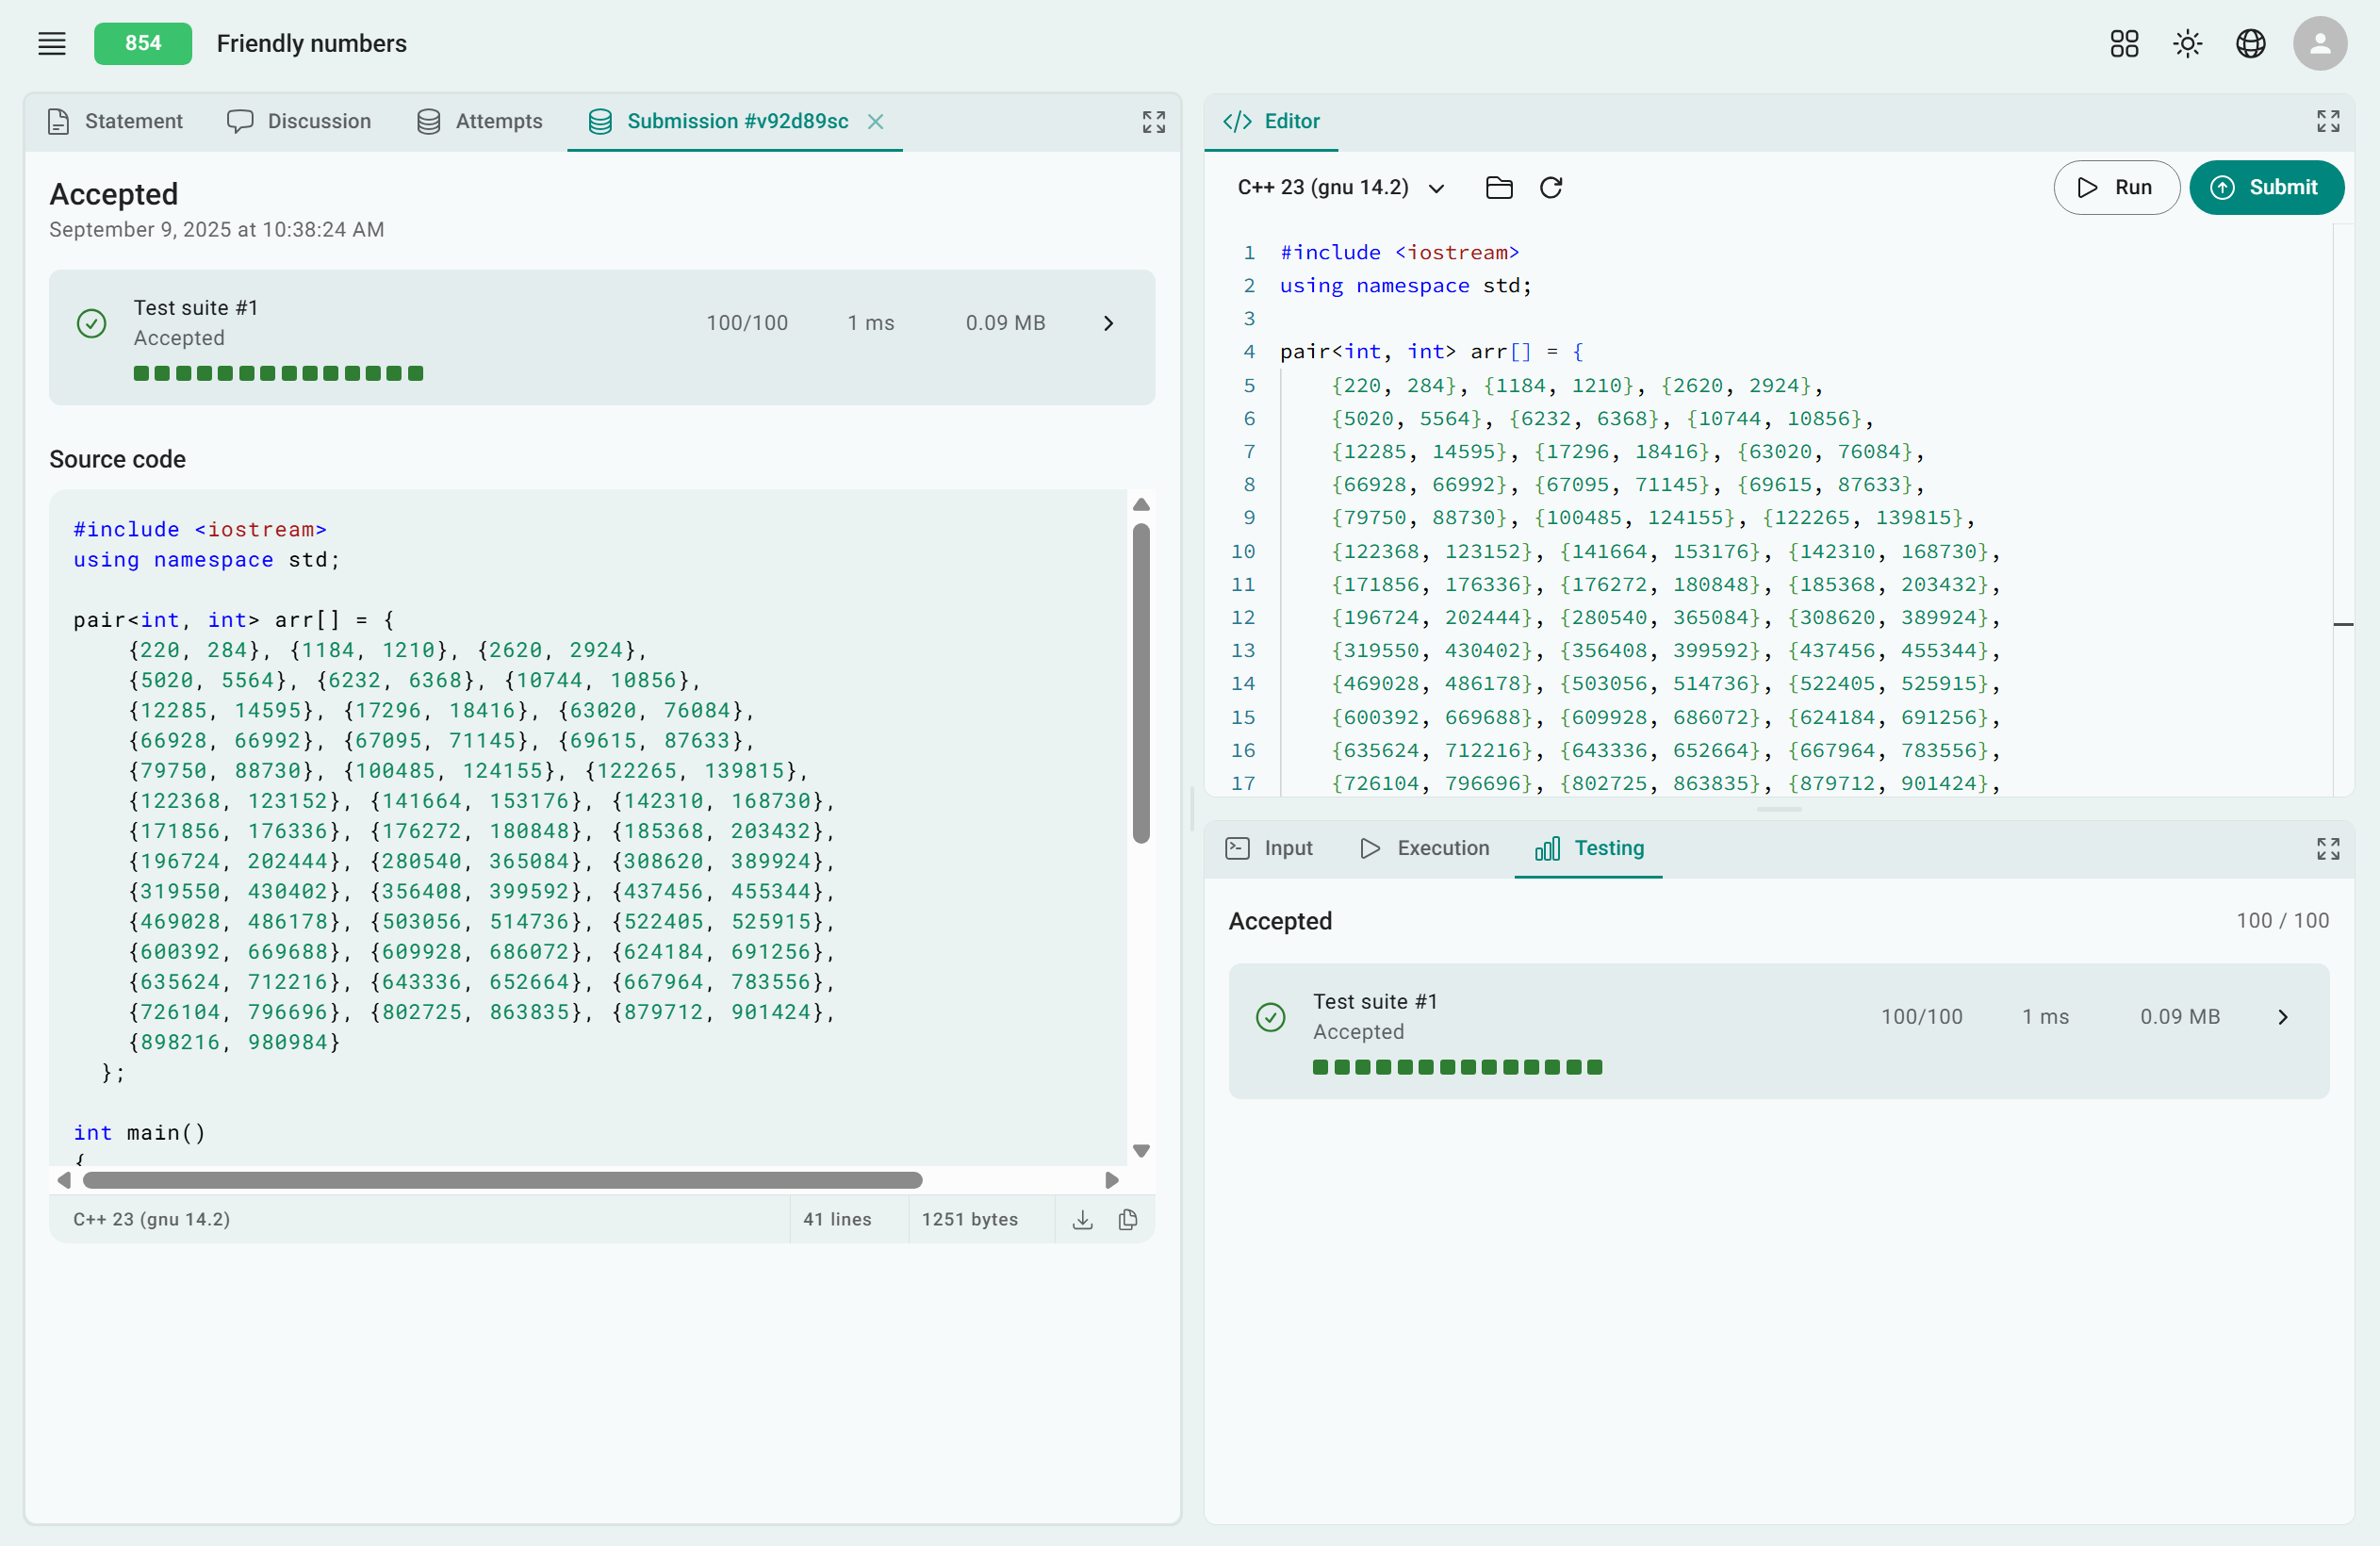
\includegraphics[scale=0.23]{img/buktiAC.png}

\section{Referensi}
\begin{itemize}
  \item Soal: \url{https://eolymp.com/en/problems/854}
  \item Wikipedia: \url{https://en.wikipedia.org/wiki/Amicable_numbers}
\end{itemize}

\end{document}